\documentclass[11pt]{article}


\setlength{\parindent}{0pt}
\usepackage{xltxtra}
\usepackage{hyperref}
\hypersetup{hidelinks}
\usepackage{url}
\urlstyle{tt}
\usepackage{xcolor}
\definecolor{CVBlue}{RGB}{23,110,191}
\usepackage{calc}
\usepackage{graphicx}
\usepackage{tikz}
\usetikzlibrary{calc}
\usepackage{fontspec}
\usepackage{xeCJK}
\usepackage{enumitem}
\CJKsetecglue{} %% 取消中文与数字之间的间隙


%% 主文档字体设置
\setmainfont[
    Path = fonts/Main/,
    Extension = .otf,
    BoldFont = texgyretermes-bold.otf, % 加粗字体
]{texgyretermes-regular.otf} % 正文字体

% 中文字体设置
\setCJKmainfont[
    Path = fonts/hansans/,
    Extension = .ttf,
    BoldFont = NotoSansSC-Bold.ttf, % 加粗字体
]{NotoSansSC-Regular.otf} % 正文字体


\usepackage{relsize}
\usepackage{xspace}

% 使用 fontawesome（部分图标）
\usepackage{fontawesome} 

% A4纸，上下左右边距
\usepackage[
    a4paper,
    left=1.2cm,
    right=1.2cm,
    top=1.5cm,
    bottom=1cm,
    nohead
]{geometry}

\renewcommand{\baselinestretch}{1.5} % 行间距设为1.5

\usepackage{titlesec}
\usepackage{enumitem}
\setlist{noitemsep} % 取消列表项间的额外间距
%\setlist{nosep} % 取消所有垂直间距
\setlist[itemize]{topsep=0.25em, leftmargin=*}
\setlist[enumerate]{topsep=0.25em, leftmargin=*}

% --- 用于控制【不同项目之间】的垂直距离 ---
\newlength{\interProjectSpacing}
\setlength{\interProjectSpacing}{0.9em} % <--- 在此调整项目之间的距离
\newcommand{\projectsep}{\vspace{\interProjectSpacing}}

% --- 用于控制【项目标题】与下方【项目描述】的距离 ---
\newlength{\intraProjectTitleSep}
\setlength{\intraProjectTitleSep}{0.4em} % <--- 在此调整标题和描述的距离
\newcommand{\titlebreak}{\\[\intraProjectTitleSep]}

% --- 用于控制【项目描述】与下方【要点列表】的距离 ---
\newlength{\intraProjectListTopSep}
\setlength{\intraProjectListTopSep}{0.2em} % <--- 在此调整描述和列表的距离

% =======================================================================


\titleformat{\section}         % 定制 \section 命令 
{\large\bfseries\raggedright} % 将 section 标题设置为大号、粗体且左对齐
{}{0em}                      % 可用于为所有 section 添加前缀（如“章节...”）
{}                           % 可用于在标题前插入代码
[{\color{CVBlue}\titlerule}]  % 在标题后插入一条横线
\titlespacing*{\section}{0cm}{*1.6}{*1.2}



\begin{document}
\pagenumbering{gobble}

%%%% 利用tikz来定位照片
\begin{tikzpicture}[remember picture, overlay] 
    \node[anchor = north east] at ($(current page.north east)+(-2cm,-1.2cm)$) {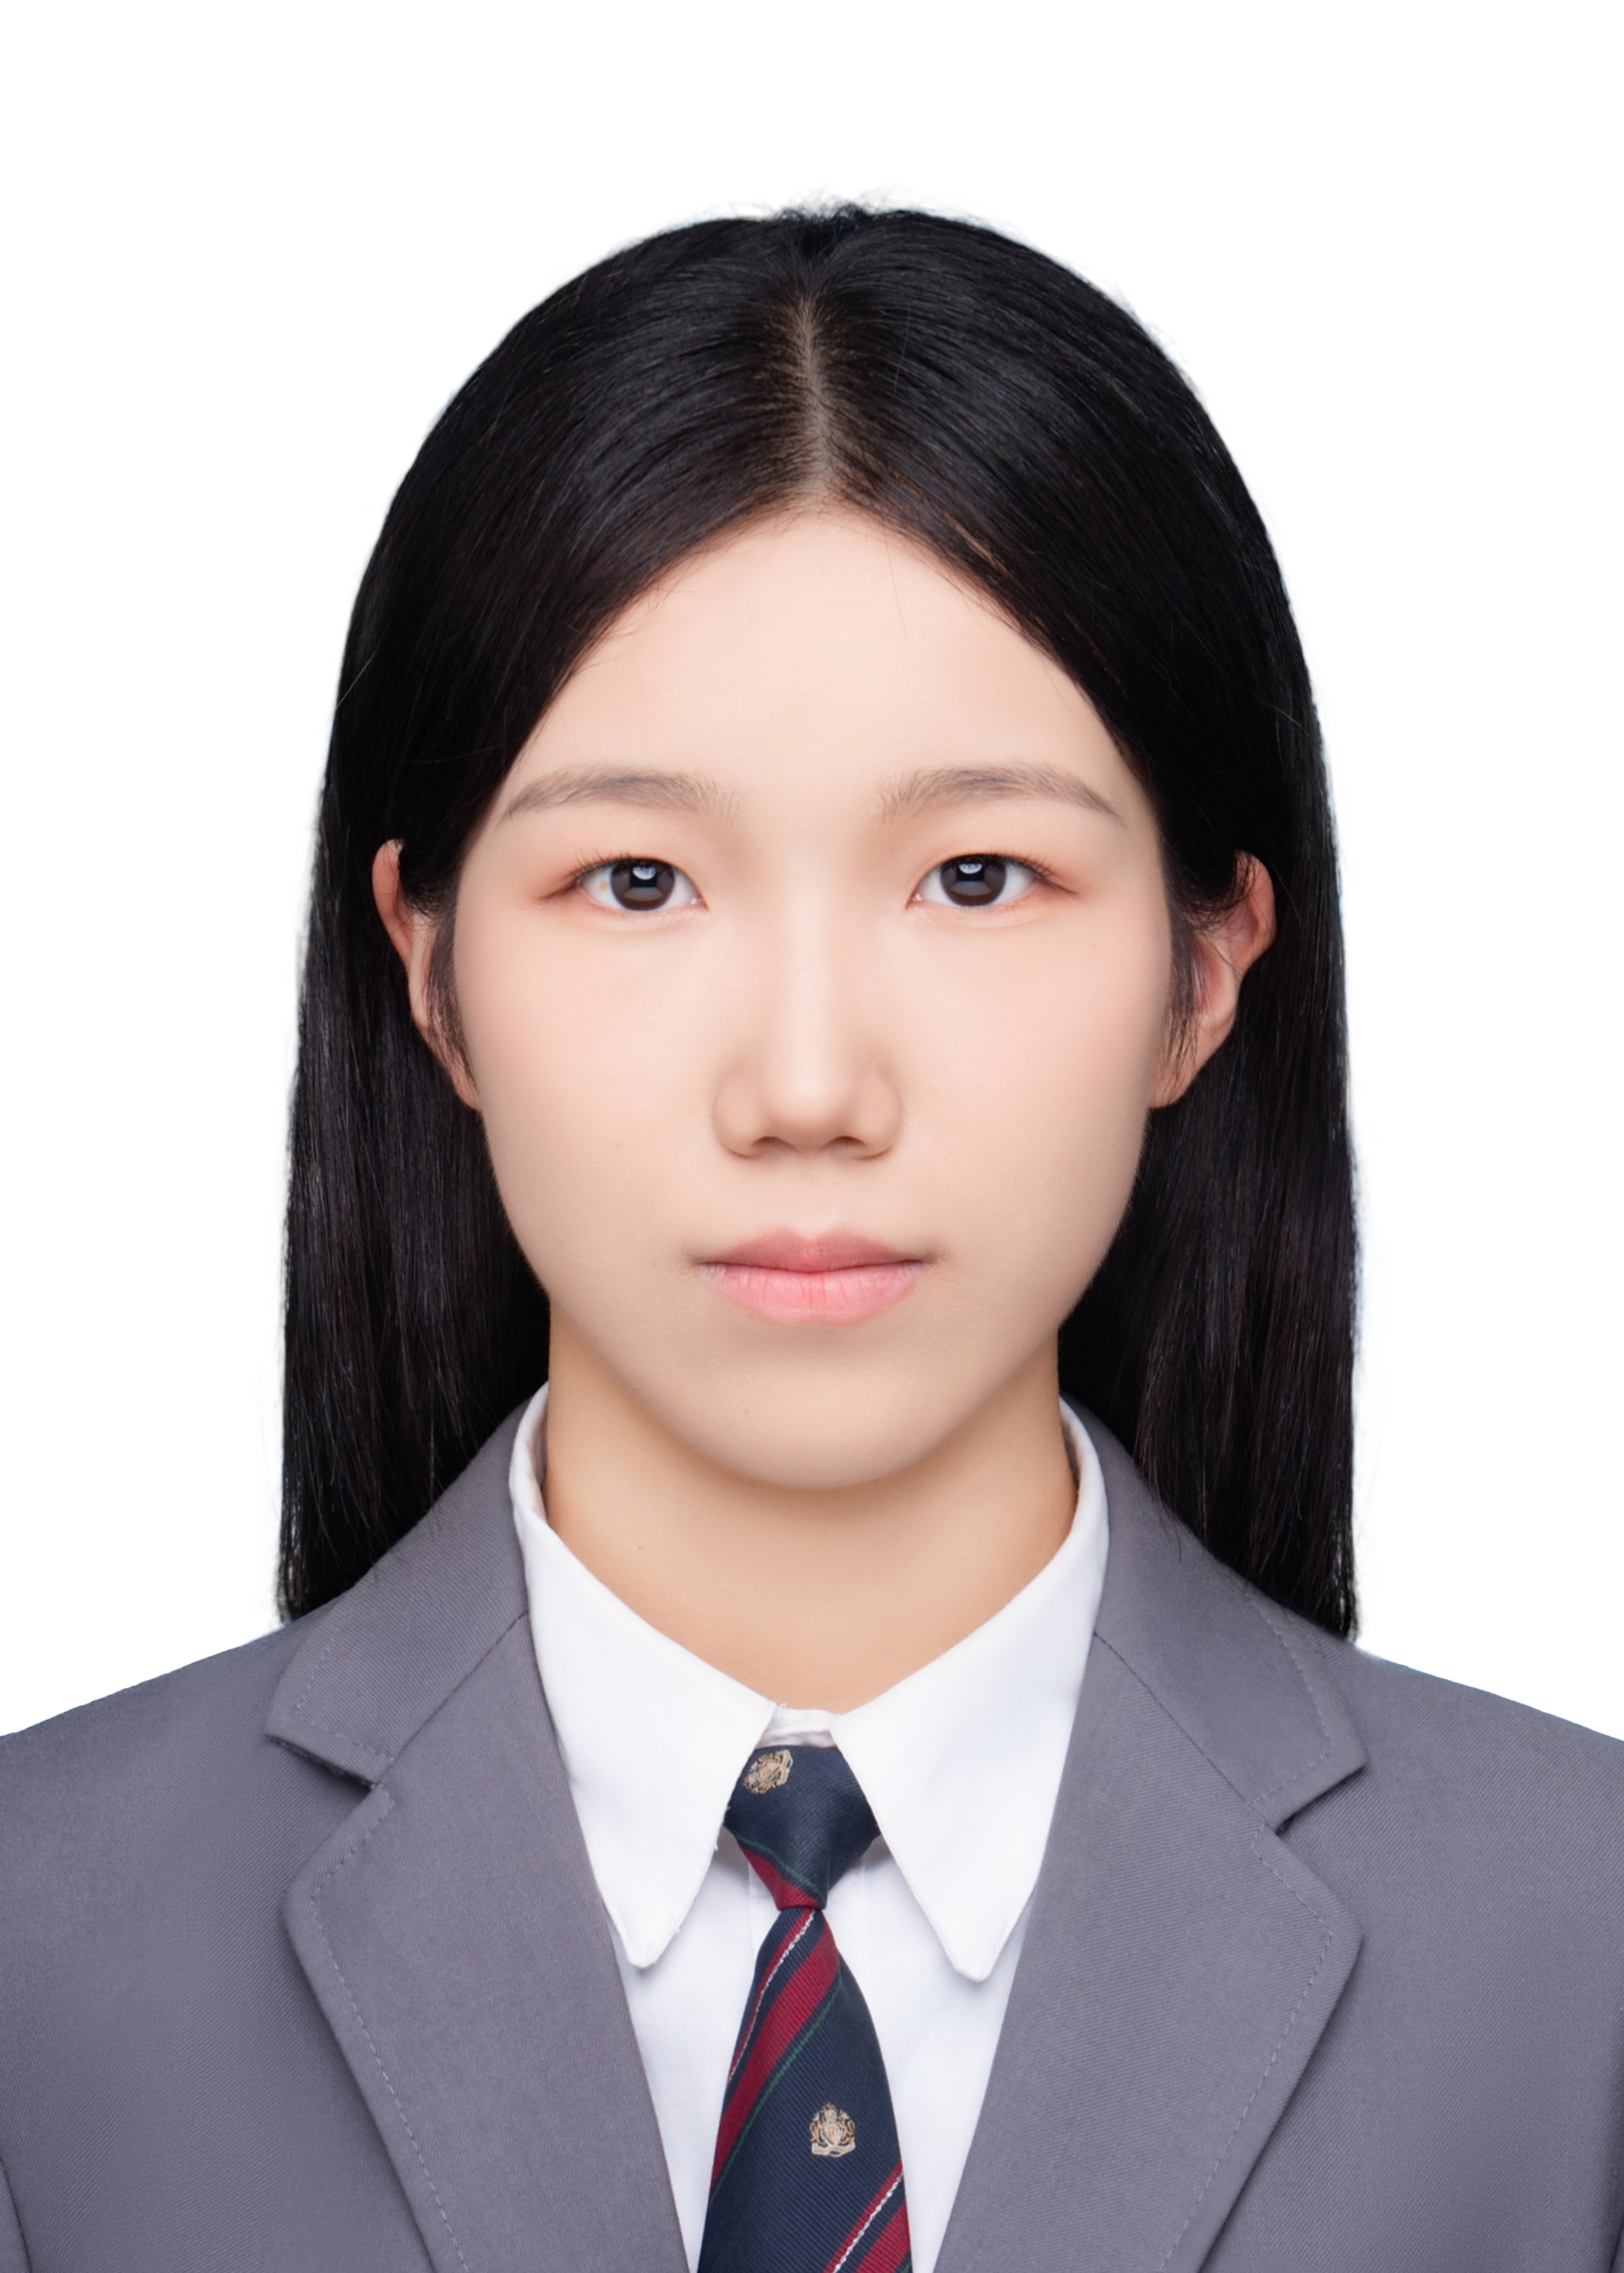
\includegraphics[height=3cm]{CV-W.jpg}};
  \end{tikzpicture}%
  %%%% 利用tikz来定位学校Logo，这里只在第一页显示
  \begin{tikzpicture}[remember picture, overlay] 
    \node[anchor = north west] at ($(current page.north west)+(0.5cm,+1.0cm)$) {\includegraphics[height=6cm]{zju.png}};
  \end{tikzpicture}%
\centerline{\LARGE\bfseries{沈璐瑶}} 

\centerline{\normalsize{\faPhone\ 152-5753-5173 \quad \faEnvelopeO\ \href{mailto:3250100324@zju.edu.cn}{3250100324@zju.edu.cn}}} 

\centerline{\normalsize{\faGithubSquare\ \href{https://github.com/shenluyao}{https://github.com/shenluyao} \quad \faRssSquare\ \href{https://sly0413.vercel.app/}{https://sly0413.vercel.app/}}} 
    
\section{\makebox[\widthof{\faGraduationCap}][c]{\color{CVBlue}\faGraduationCap}\ 教育背景}    
\textbf{浙江大学} \hfill 2025.9 -- 至今\\[-1.8em] % 标题和正文间加一点距离
\begin{itemize}[nosep]
    \item \textbf{平均绩点}：4.66/5.0，\textbf{工信大类排名}: 24/757
    \item 相关课程及成绩：《线性代数（甲）》 94/4.8、《C程序设计基础及实验》 92/4.8
\end{itemize}
\textbf{浙江省春晖中学} \hfill 2022.9 -- 2025.7\\[-1.8em]
\begin{itemize}[nosep]
    \item 相关荣誉及奖项：校级三好学生、市化学竞赛二等奖、市物理竞赛一等奖
\end{itemize}

\section{\makebox[\widthof{\faUsers}][c]{\color{CVBlue}\faUsers}\ 项目经历}

% --- 第一个项目 ---
% 将标题行末尾的 \\ 替换为 \titlebreak 命令

\textbf{离线版WikiRacer} \hfill 2026.01 \titlebreak
项目描述：来自UCB CS106L的project,给定两个维基词条，在维基百科链接构成的词网中自动求解从起点到终点的最短路径。
\begin{itemize}[nosep, topsep=\intraProjectListTopSep]
    \item \textbf{技术栈}：C++, QtCreator
\end{itemize}

\projectsep

\textbf{MNIST手写体识别模型复现} \hfill 2026.02 \titlebreak
项目描述：实现的一个简单的神经网络，在MNIST数据集上进行训练和测试，达到较高的识别准确率。
\begin{itemize}[nosep, topsep=\intraProjectListTopSep]
    \item \textbf{技术栈}：PyTorch,Google Colab
\end{itemize}

\projectsep

\textbf{搭建个人学习网站} \hfill 2026.02 \titlebreak
项目描述：用于管理个人笔记、记录每日学习任务，并对页面访问人次进行统计。
% 在 itemize 的选项中，使用 topsep=\intraProjectListTopSep 来控制上边距
\begin{itemize}[nosep, topsep=\intraProjectListTopSep]
    \item \textbf{技术栈}：Next.js 16, React 10, TypeScript, Supabase,Vercel
\end{itemize}

% 使用 \projectsep 命令来分隔两个项目
\projectsep

% --- 第二个项目 ---
\textbf{AnyCar-四路红外小车循迹项目} \hfill 2025.11-2025.12 \titlebreak
项目描述：一款四路红外小车循迹系统。支持PID巡线、直角弯识别与终点黑框检测，实现自动寻迹与停车。
\begin{itemize}[nosep, topsep=\intraProjectListTopSep]
    \item \textbf{技术栈}：Arduino，C语言，L298N双电机驱动，数字I/O与PWM调速，串口调试
\end{itemize}

\section{\makebox[\widthof{\faCogs}][c]{\color{CVBlue}\faCogs}\ 技术栈}
\begin{itemize}[nosep]
    \item \textbf{编程语言：} C语言, Python, C++
    \item \textbf{开发工具：} Git, Visual Studio Code, QtCreator, PyCharm
\end{itemize}
\section{\makebox[\widthof{\faGraduationCap}][c]{\color{CVBlue}\faList}\ 英语水平}
\begin{itemize}
    \item 《大学英语 III》 90/4.5
    \item 浙江英语高考 140
    
\end{itemize}
    
\section{\makebox[\widthof{\faInfo}][c]{\color{CVBlue}\faInfo}\ 学生工作及社团经历}
\begin{itemize}[parsep=0.5ex]
    \item \textbf{云峰分团委：} 担任分团委实践部干事，参与组织暑期社会实践结项答辩、云峰十佳答辩
    \item \textbf{机器人协会：} 担任协会组织部干事，参与组织湖州开放日活动；参与内训、巡线小车项目开发
\end{itemize}
\end{document}


